%
% Apunte de Sistemas Operativos
% Copyright (C) 2014 Esteban De La Fuente Rubio (esteban[at]delaf.cl)
%
% Permission is granted to copy, distribute and/or modify this document
% under the terms of the GNU Free Documentation License, Version 1.3
% or any later version published by the Free Software Foundation;
% with no Invariant Sections, no Front-Cover Texts, and no Back-Cover Texts.
% A copy of the license is included in the section entitled "GNU
% Free Documentation License".
%
% Link: http://www.gnu.org/copyleft/fdl.html
%

% WARNING: caracteres especiales (como eñes y acentos) han sido omitidos a
% propósito al utilizar lstlisting, ya que este paquete no soporta UTF-8.

% SINCRONIZACIÓN
\chapter{Sincronización}
\label{sincronizacion}

Este capítulo se centra en mecanismos de sincronización entre procesos, esto
con el objetivo de solucionar los problemas descritos anteriormente:
\emph{dataraces}, \emph{deadlock} y \emph{starvation}.

Se mostrará primero la forma incorrecta de solucionar los problemas de exclusión
mutua, utilizando \emph{busy-waiting}. Luego se presentarán los problemas
clásicos estudiados en sistemas operativos, estos son ``productor consumidor'',
``cena de filósofos'' y ``lectores escritores''. Finalmente se introducirán tres
herramientas de sincronización, las cuales corresponden a semáforos, monitores y
mensajes.

\section{\emph{Busy-waiting}}
Una solución a los problemas de exclusión mutua es consultar reiteradamente si
el recurso que se está solicitando está o no disponible. Son interesantes, ya
que permiten entender porque son incorrectas y que las hace inapropiadas para el
problema de exclusión mutua.

Una de las posibles soluciones es utilizar una bandera o \emph{flag} para
indicar si la sección crítica esta (1) o no (0) siendo ocupada.

\begin{lstlisting}
int bandera = 0;
int contador = 0;
void aumentar()
{
	while (bandera);
	bandera = 1;
	int aux = contador;
	contador = aux + 1;
	bandera = 0;
}
\end{lstlisting}

\begin{enumerate}[a)]

\item \textbf{¿Qué sucede con la variable global bandera?} al ser compartida y
accedida (para lectura y modificación) por más de un proceso se convierte
también  en una sección crítica vulnerable \emph{data races}. O sea, lo que
se pretendía usar para controlar a sección crítica se convierte en una sección
rítica.                                                         
	
\item \textbf{¿Qué ocurre si dos procesos consultan en el \texttt{while} y la
bandera es 0?} Puede ocurrir que el primer proceso sea interrumpido justo
después del \texttt{while} y, al no alcanzar a poner la bandera en 1, el segundo
proceso también entre a la sección crítica que se quiere proteger.
	
\end{enumerate}

Existen diversas soluciones para el problema de exclusión mutua utilizando
\emph{busy-waiting}. Se pueden revisar los algoritmos de Dekker y Peterson
para más soluciones de este tipo.

El gran problema con las soluciones de \emph{busy-waiting} es que realizan una
\textbf{espera activa} del recurso. Esto significa que utilizan CPU para
consultar cada vez por el recurso. Lo que se verá en el resto del capítulo serán
herramientas de sincronización con \emph{espera pasiva}, donde el proceso
consulta, y si el recurso está ocupado se ``duerme''.

Es importante destacar que la espera activa es el problema de todas las
soluciones que utilizan \emph{busy-waiting}, sin embargo pueden existir
soluciones de este tipo que a pesar de este problema sean correctas para
realizar la sincronización.

\section{Problemas clásicos}
En la literatura relacionada con sistemas operativos generalmente se mencionan
tres problemas clásicos, los cuales se enunciarán a continuación y serán
utilizados durante los ejemplos de los diferentes métodos de sincronización.

\subsection{Productor consumidor}
En el problema del productor consumidor, o \emph{buffer} acotado, existe uno o
varios productores que \textbf{producen cierto elemento} mientras que uno o
varios consumidores \textbf{consumen dicho elemento}. Las operaciones
\emph{put} y \emph{get} se realizan sobre una pila finita y los
elementos deben ser entregados en el mismo orden en que fueron depositados.

A continuación se muestra una visión global del problema, posteriormente una
solución incorrecta. Soluciones correctas serán vistas cuando se estudien los
diferentes mecanismos de sincronización.

Versión secuencial (no interesante):
\begin{lstlisting}
void productor_consumidor ()
{
  for (;;) {
    item it = produce();
    consume(it);
  }
}
\end{lstlisting}

Versión paralela (interesante):
\begin{lstlisting}
void productor ()
{
  for (;;) {
    item it = produce();
    put(it);
  }
}
void consumidor ()
{
  for (;;) {
    item it = get();
    consume(it);
  }
}
\end{lstlisting}

Restricciones:
\begin{itemize}

\item \emph{get} no puede entregar \emph{items} que no fueron suministrados
con \emph{put} (se deberá bloquear el consumidor si no hay items).
	
\item Con \emph{put} se pueden recibir hasta $N$ \emph{items} sin que hayan
sido extraídos con \emph{get} (se deberá bloquear del productor si la pila
está llena).

\item \emph{Items} tienen que ser extraídos en el mismo orden en que fueron
depositados.

\item Tiene que funcionar en paralelo (no sirve versión secuencial).

\end{itemize}

Las funciones \emph{produce} y \emph{consume} son lentas y pueden ser
ejecutadas en paralelo sin ningún problema (ya que no interactuan al mismo
tiempo con otros procesos sobre algún recurso compartido). La solución deberá
considerar la implementación sincronizada de \emph{put} y \emph{get},
asumiendo el resto de funciones como dadas (o sea, existen y funcionan).

\begin{figure}[htbp]
	\centering
	\selectlanguage{english}
	\begin{tikzpicture}
		% formatos
		\tikzstyle{productor} = [draw, circle, node distance=4cm]
		\tikzstyle{consumidor} = [draw, circle, node distance=4cm]
		\tikzstyle{stack} = [draw, rectangle split, rectangle split
horizontal, rectangle split parts=10]
		\tikzstyle{arrow} = [->, semithick, auto]
		% productores y consumidores
		\node [productor]  (P1)
	  {P1};
		\node [productor]	 (P2)	[right of =P1]	{P2};
		\node [consumidor] (C1)	[right of =P2]	{C1};
		\node [consumidor] (C2) [right of =C1]  {C2};
		% stack
		\node at (6, -2) [stack] (stack) {
			\nodepart{six}X
			\nodepart{seven}X
		};		
		% relaciones
		\draw [arrow] (P1) to node {put} (stack);
		\draw [arrow] (P2) to node {put} (stack);
		\draw [arrow] (stack) to node {get} (C1);
		\draw [arrow] (stack) to node {get} (C2);
	\end{tikzpicture}
	\selectlanguage{spanish}
	\caption{Interacción entre productores y consumidores}
	\label{fig:interaccion_productores_consumidores}
\end{figure}

\subsubsection{Solución incorrecta: \emph{data races}}

\begin{lstlisting}
#define N 100
Item buffer[N];
int e = 0;
int f = 0;
int c = 0;
void put (Item item)
{
  while(c==N);
  buffer[e] = item;
  e = (e+1) % N;
  c++;
}
Item get ()
{
  Item item;
  while(c==0);
  item = buffer[f];
  f = (f+1) % N;
  c--;
  return item;
}
\end{lstlisting}

\textbf{¿Por qué la solución anterior es incorrecta?} Al utilizar una variable
global $c$ para indicar la cantidad de elementos que hay en la pila, se incurre
en el problema de exclusión mutua, donde si no hay sincronización la variable
$c$ podría sufrir problemas de \emph{data races} y quedar en un estado
inconsistente durante algún punto de la ejecución. Adicionalmente la solución
considera el uso de \emph{busy-waiting} lo cual ya se discutió que no es
aceptable.

\subsection{Cena de filósofos}
Se ha invitado a una cena a cinco filósofos chinos a comer y pensar, donde
realizan solo una de estas actividades al mismo tiempo. En la mesa donde se han
de sentar existen 5 puestos y 5 palitos (o tenedores, dependiendo de la
bibliografía).

\begin{figure}[htbp]
\centering
\includegraphics[scale=1.00]{img/C05_sincronizacion/filosofos.png}
\caption{Problema cena de filósofos}
\label{fig:concurrencia_filosofos}
\end{figure}

Restricciones:
\begin{itemize}
\item Cada filósofo solo puede tomar palitos que están a su lado.
\item Un filósofo requiere dos palitos para comer.
\item Un palito no puede ser utilizado por dos filósofos al mismo tiempo.
\end{itemize}

\subsubsection{Solución incorrecta: \emph{data races}}
\begin{lstlisting}
void filosofo (int i)
{
  for(;;) {
    comer(i, (i+1)%5);
    pensar();
  }
}
\end{lstlisting}

El problema en esta solución ocurre por el uso de la función comer
directamente con $i$ e $i+1$, dos filósofos podrían tomar el mismo palito.

\subsection{Lectores escritores}
Este problema utiliza la idea de un diccionario, se dispone de dos arreglos de
tamaño fijo donde uno contiene las palabras del diccionario y el otro sus
definiciones. Se mostrarán los prototipos (o firmas) de funciones para poder
agregar una nueva definición al diccionario, para consultar por una definición y
para eliminar una definición.

Restricciones:
\begin{itemize}
\item $n$ lectores o escritores requieren acceso a una estructura de datos
compartida.
\item Los lectores solo consultan.
\item Los escritores modifican la estructura de datos.
\item Lectores y escritores deberán utilizar herramientas de sincronización ya
que si bien múltiples lectores pueden trabajar sobre la estructura, solo un
escritor puede hacerlo en un determinado tiempo.
\end{itemize}

Suponga la siguiente API:
\begin{lstlisting}
void newDef (char *k, char *d);
char *query (char *k);
void delDef (char *k);
\end{lstlisting}

Un ejemplo del uso de la API se ilustra a continuación:
\begin{lstlisting}
newDef("a", "1");           /* se crea palabra "a" con definicion "1" */
printf("%s\n", query("a")); /* imprime: 1 */
delDef("a");                /* se elimina la palabra a */
printf("%s\n", query("a")); /* NULL */
\end{lstlisting}

Se debe implementar la API de tal forma de cumplir con los requisitos y
restricciones del problema.

\subsubsection{Solución incorrecta: \emph{data races}}
\begin{lstlisting}
/* Definicion de arreglos globales para palabras y definiciones */
#define MAX 100
char *keys[MAX], *defs[MAX];

/* Funcion que obtiene una casilla vacia */
int getSlot ()
{
  int i;
  for(i=0; i<MAX; i++)
    if(keys[i]==NULL)
      return i;
  return -1;
}

/* Funcion que crea una nueva definicion en el diccionario */
void newDef (char *k, char *d)
{
  int i = getSlot();
  if(i!=-1) {
    keys[i] = k;
    defs[i] = d;
  }
}

/* Funcion que obtiene la posicion en la casilla a partir de una clave */
int getIdX (char *k)
{
  int i;
  for(i=0; i<MAX; i++)
    if(keys[i]!=NULL && !strcmp(k, keys[i]))
      return i;
  return -1;
}

/* Funcion que recupera una definicion */
char *query (char *k)
{
  int i = getIdX(k);
  return i==-1 ? NULL : defs[i];
}

/* Funcion que elimina una definicion del diccionario */
void delDef (char *k)
{
  int i = getIdX(k);
  if(i!=-1) {
    keys[i] = NULL;
    defs[i] = NULL;
  }
}
\end{lstlisting}

Al analizar el código se observa que pueden ocurrir \emph{data races} si se
realizan al menos dos modificaciones en paralelo o si se realiza una
modificación con una consulta. No ocurrirán problemas si se realizan dos
consultas en paralelo.

Algunas de las situaciones anómalas se describen a continuación (el lector
deberá considerar que otros problemas pueden ocurrir).

\begin{enumerate}[i.]

\item \textbf{\texttt{newDef} con \texttt{newDef}}: al realizar una nueva
definición se consulta por una casilla libre, si justo en el momento después de
consultar si la casilla está libre (instrucción \texttt{if} en
\texttt{getSlot}), se saca al proceso de la CPU y entra otro proceso que hace la
misma consulta se podría entregar la misma casilla a ambos procesos.

\item \textbf{\texttt{query} con \texttt{delDef}}: al seleccionar una
definición se consulta mediante \texttt{getIdX} el índice dentro del arreglo, si
justo después de consultar por el índice se saca al proceso de la CPU y se llama
a \texttt{delDef} eliminando la misma definición consultada, cuando
\texttt{query} retome la CPU y use el índice obtenido no estará lo esperado en
la casilla.

\item \textbf{\texttt{query} con \texttt{newDef}}: el resultado de
\texttt{query} puede ser \texttt{NULL} si se ejecuta antes que \texttt{newDef} o
distinto de \texttt{NULL} si se ejecuta después.

\end{enumerate}

\section{Semáforos}
Los \textbf{semáforos} corresponden básicamente a contadores (de
\emph{tickets}), donde para utilizar una sección crítica se consulta por el
valor del semáforo, si este es mayor a cero (o sea hay tickets) se usa la
sección, si es igual a cero, se deberá esperar.

El valor del semáforo (o la cantidad de tickets) será inicializado,
generalmente, en la cantidad de procesos que pueden hacer uso al mismo tiempo de
la sección crítica. Adicionalmente las rutinas utilizadas deben ser atómicas,
esto para garantizar que varios procesos puedan consultar el valor del semáforo
sin que ocurran \emph{data races}.

\begin{lstlisting}
s=1;
void proceso ()
{
 solicitar_ticket(s);
 // ejecucion de seccion critica
 liberar_ticket(s);
}
\end{lstlisting}

Los procesos que no tengan acceso al semáforo, por falta de \emph{tickets},
deberán esperar en una cola FIFO a que se depositen \emph{tickets}, en cuyo
momento se despertará al proceso que estaba primero en la cola para que obtenga
el \emph{ticket} del semáforo y entre en la sección crítica.

\subsection{API}

\begin{lstlisting}
/* Inicializa el semaforo */
struct semaphore *semaphore_make (int tickets);

/* Solicita el semaforo */
void semaphore_wait (struct semaphore *s);

/* Libera el semáforo */
void semaphore_signal (struct semaphore *s);
\end{lstlisting}

\subsection{Modo de operación}
Un bosquejo de la implementación de las funciones de la API que ayudará a
comprender como operan los semáforos es la siguiente:

\begin{lstlisting}
void wait (s)
{
  s--;
  if(s < 0)
    block(s);     /* suspender proceso y agregarlo al final de la cola */
}
void signal (s)
{
  s++;
  if (s <= 0)
    wakeup(s);    /* despertar primer proceso en la cola */
}
\end{lstlisting}

\textbf{¿Qué significa que el valor del semáforo sea -1?}, significaría que ya
hay un proceso antes en la cola FIFO. Por lo cual al recibir un \texttt{signal}
se despertará primero al otro proceso.

Una implementación real, utilizando \texttt{nSystem}\footnote{Sistema
Operativo de juguete desarrollado por el profesor Luis Mateu de la Universidad
de Chile}, puede ser vista en el anexo \ref{nSystem}.

\subsection{Problema productor consumidor}

\subsubsection{Solución correcta}

\begin{lstlisting}
#define N 100
Item buffer[N];
int e = 0;
int f = 0;
struct semaphore *empty; /* = semaphore_make (0) */
struct semaphore *full;  /* = semaphore_make (N) */
void put (Item item)
{
  semaphore_wait (empty);
  buffer[e] = item;
  e = (e+1) % N;
  semaphore_signal (full);
}
Item get ()
{
  Item item;
  semaphore_wait (full);
  item = buffer[f];
  f = (f+1) % N;
  semaphore_signal (empty);
  return item;
}
\end{lstlisting}

Esta solución es válida para un productor y un consumidor. Para $n$ productores
y $m$ consumidores se debe definir un semáforo adicional para cubrir la sección
crítica tanto de la función \texttt{put} como de la función \texttt{get}. Esto
queda de tarea al lector.

\subsection{Problema cena de filósofos}

\subsubsection{Solución incorrecta: \emph{deadlock}}

\begin{lstlisting}
struct semaphore s[5]; /* for(i=0; i<5; i++) s[i] = semaphore_make (1); */
void filosofo (int i)
{
  for(;;) {
    semaphore_wait (s[i]);
    semaphore_wait (s[(i+1)%5]);
    comer (i, (i+1)%5);
    semaphore_signal (s[i]);
    semaphore_signal (s[(i+1)%5]);
    pensar ();
  }
}
\end{lstlisting}

El problema en esta solución es lo que sucedería si todos los filósofos
solicitaran el palito $i$ ``al mismo tiempo'', cuando quieran solicitar el
palito $i+1$ ya alguien lo tendrá tomado.

\subsubsection{Solución correcta específica}
Se debe evitar que entren los 5 filósofos al mismo tiempo a la mesa, con esto se
asegurará que al menos uno de ellos coma. En este caso la misma mesa se
convierte en una sección crítica.

\begin{lstlisting}
struct semaphore *m;    /* m = semaphore_make (4); */
struct semaphore s[5];  /* for(i=0; i<5; i++) s[i] = semaphore_make (1); */
void filosofo (int i)
{
  for(;;) {
    semaphore_wait (m);
    semaphore_wait (s[i]);
    semaphore_wait (s[(i+1)%5]);
    comer (i, (i+1)%5);
    semaphore_signal (s[i]);
    semaphore_signal (s[(i+1)%5]);
    semaphore_signal (m);
    pensar ();
  }
}
\end{lstlisting}

\subsubsection{Solución correcta general}
Se deben solicitar los recursos siempre en el mismo orden, ya sea ascendente o
descendente. Esto evitará el interbloqueo.

\begin{lstlisting}
struct semaphore s[5];  /* for(i=0; i<5; i++) s[i] = semaphore_make (1); */
void filosofo (int i)
{
  int min = min (i, (i+1)%5);
  int max = max (i, (i+1)%5);
  for(;;) {
    semaphore_wait (s[min]);
    semaphore_wait (s[max]);
    comer(min, max);
    semaphore_signal (s[min]);
    semaphore_signal (s[max]);
    pensar();
  }
}
\end{lstlisting}

Asumamos que entra el filósofo 2, solicitará el palito 2 y el palito 3 y comerá.
Luego entra el filósofo 1, solicita el palito 1 (está disponible), pero al pedir
el palito 2 (que esta ocupado por el filósofo 2) se bloquea a la espera que se
desocupe. El problema aquí es que el filósofo 1 espera reteniendo el palito 1,
entonces si llega un filósofo 0, que puede usar el palito 0, el palito 1 no lo
conseguirá a pesar de que no está siendo utilizado para comer (solo está siendo
retenido por el filósofo 1). Eventualmente, cuando el filósofo 2 libere el
palito 2, el filósofo 1 comerá y eventualmente el 0 también lo hará. Sin embargo
¿podría haber comido el 2 y el 0 al mismo tiempo?, la respuesta es sí.

El problema de los semáforos, en general, es que no se puede saber si el
semáforo está o no ocupado antes de pedirlo. Esto trae como consecuencia una
limitación del paralelismo, ya que al consultar por el palito este es retenido
independientemente de si el otro está o no disponible. Sin embargo, si se
considera que la operación comer es mucho más rápida que la de pensar, por
ejemplo asumiendo que comer es leer datos y pensar es procesarlos, esta
limitación de paralelismo no es tan grave para ciertos problemas.

Lo anterior se podría solucionar implementando ``algo'' que permita pedir dos
semáforos al mismo tiempo, pero que no los deje tomados si uno de ellos está
ocupado. Esto entregará un mayor paralelismo, pero introducirá el problema de
hambruna, donde dos filósofos (por ejemplo filósofos 0 y 2) podrían estar
pidiendo siempre los palitos que un tercero (filósofo 1) quisiera utilizar.

\section{Monitores de Brinch Hansen}
Los \textbf{monitores} de Brinch
Hansen\footnote{\url{http://es.wikipedia.org/wiki/Per_Brinch_Hansen}} son una
herramienta de sincronización que ofrece más paralelismo que los semáforos, pero
pueden provocar hambruna. Permitirán consultar al mismo tiempo por el valor de
más de una condición, si alguno de los elementos de dicha condición no se cumple
de la forma requerida el proceso se suspenderá.

Los monitores pueden ser vistos como semáforos binarios, donde el
``\emph{ticket}'' del monitor es la propiedad del mismo.

\begin{lstlisting}
void proceso ()
{
 solicitar_propiedad(m);
 // ejecución de sección crítica
 liberar_propiedad(m);
}
\end{lstlisting}

Es importante mencionar que la propiedad del monitor debe ser devuelta siempre
por el mismo proceso que la solicitó.

\subsection{API}

\begin{lstlisting}
/* Crear un monitor */
struct monitor *monitor_make ();

/* Destruir un monitor */
void monitor_destroy (struct monitor *m);

/* Solicitar la propiedad sobre un monitor */
void monitor_enter (struct monitor *m);

/* Devuelve la propiedad del monitor */
void monitor_exit (struct monitor *m);

/* Devuelve la propiedad y suspende el proceso hasta un monitor_notify_all  */
void monitor_wait (struct monitor *m);

/* Despierta las tareas suspendidas con monitor_wait  que esperan la propiedad
del monitor */
void monitor_notify_all (struct monitor *m);
\end{lstlisting}

Un proceso que espera, suspendido, por la propiedad del monitor al haber usado
\texttt{monitor\_enter} esperará hasta que esta sea liberada por el proceso que
la ocupa, ya sea mediante un \texttt{monitor\_wait} o un \texttt{monitor\_exit}.

Al despertar procesos bloqueados por un \texttt{monitor\_enter} o un
\texttt{monitor\_wait} obtendrán la propiedad sin garantía del orden, o sea,
\textbf{monitores no son FIFO}. Igualmente, cuando se hace una llamada a
\texttt{monitor\_notify\_all} se despertarán todos los procesos suspendidos
por un \texttt{monitor\_wait} del mismo monitor, el orden en que despiertan no
está garantizado, o sea no necesariamente es FIFO respecto a la ejecución de
\texttt{monitor\_wait}. Adicionalmente una vez despertados los procesos deben
esperar la propiedad del monitor (esto ya que \texttt{monitor\_notify\_all}
solo despierta, no entrega la propiedad, la cual será entregada al usar
\texttt{monitor\_exit}) y evaluar nuevamente sus condiciones, si nuevamente no
se cumplen se suspenderán liberando el monitor, así otro proceso despertado con
\texttt{monitor\_notify\_all} podrá obtener la propiedad y también evaluar sus
condiciones nuevamente. Podría ocurrir también que con
\texttt{monitor\_notify\_all} los procesos al evaluar sus condiciones, ninguno
pueda continuar, y todos se vuelvan a suspender.

\subsection{Problema productor consumidor}

\subsubsection{Solución incorrecta: \emph{deadlock}}
\begin{lstlisting}
void put (Item it)
{
  monitor_enter (monitor);
  while (c==N);
  buffer[e] = it;
  e = (e+1) % N;
  c++;
  monitor_exit (monitor);
}
Item get ()
{
  Item it;
  monitor_enter (monitor);
  while(c==0);
  it = buffer[f];
  f = (f+1) % N;
  c--;
  monitor_exit (monitor);
  return it;
}
\end{lstlisting}

Suponga que $c=N$, o sea el productor no puede depositar más \emph{items} en
la pila y debe esperar. En este caso al ejecutar \texttt{put}, se solicitará la
propiedad del monitor y el proceso quedará en el ciclo del \texttt{while}, con
espera activa y con el monitor tomado. Si llega un consumidor y solicita la
propiedad sobre el monitor para extraer un \emph{item}, lo cual es válido por
la situación descrita, no podrá hacerlo, ya que el monitor está tomado por un
productor, el cual espera (la condición de su \texttt{while}) que un consumidor
extraiga al menos un \emph{item}. En este caso se produce el problema de
interbloqueo.

\subsubsection{Solución correcta}
Se debe buscar una solución que permita devolver el monitor si la condición de
espera se cumple, esto se logra utilizando \texttt{monitor\_wait} sobre el
monitor.

\begin{lstlisting}
void put (Item it)
{
  monitor_enter (monitor);
  while(c==N)
    monitor_wait (monitor);
  buffer[e] = it;
  e = (e+1) % N;
  c++;
  monitor_notify_all (monitor);
  monitor_exit (monitor);
}
Item get ()
{
  Item it;
  monitor_enter (monitor);
  while(c==0)
    monitor_wait (monitor);
  it = buffer[f];
  f = (f+1) % N;
  c--;
  monitor_notify_all (monitor);
  monitor_exit (monitor);
  return it;
}
\end{lstlisting}

Si llega un productor y ve que la pila está llena, hará espera pasiva y
devolverá la propiedad del monitor. Análogamente si un consumidor ve que la pila
está vacía esperará de forma pasiva y devolverá la propiedad del monitor. Esta
acción de devolver la propiedad del monitor y quedar en espera pasiva es lograda
mediante \texttt{monitor\_wait}. Adicionalmente se agrega la instrucción
\texttt{monitor\_notify\_all}, la cual despertará a todos los procesos
bloqueados mediante un \texttt{monitor\_wait} de dicho monitor, obtendrán la
propiedad y podrán evaluar nuevamente la condición de espera, si no se sale del
\texttt{while} se volverá a dormir entregando la propiedad a otro proceso para
que pueda continuar. Notar que no se puede determinar en que orden serán
despertados los procesos, por lo cual cualquier proceso podría tomar la
propiedad una vez sean despertados por \texttt{monitor\_notify\_all}.

\subsection{Patrón de solución usando monitores}

\begin{lstlisting}
... operacion (...)
{
  ...
  monitor_enter (m);
  while (!invariante)       /* condicion para quedar en espera */
    monitor_wait (m);
  ...                       /* operaciones */
  monitor_notify_all (m);   /* opcional, solo si las operaciones modifican
                               datos que afecten la condicion de otros que
			       esperan (además podría ir antes del while)
			     */
  monitor_exit (m);
  return ...;
}
\end{lstlisting}

Se recomienda aislar los distintos aspectos de la solución, separando el código
de sincronización del resto de la aplicación. Se verá esto a continuación en la
solución de la cena de filósofos.

\subsection{Problema cena de filósofos}
\subsubsection{Solución ``correcta''}
\begin{lstlisting}
/* llamadas a rutinas del filosofo */
void filosofo (int i)
{
  for(;;) {
    pedir (i, (i+1)%5);
    comer (i, (i+1)%5);
    devolver (i, (i+1)%5);
    pensar ();
  }
}

/* sincronizacion */

struct monitor *m;            /* m = monitor_make (); */
int ocup[5] = {0, 0, 0, 0, 0} /* =0 palito esta libre */

void pedir (int i, int j)
{
  monitor_enter (m);
  while(ocup[i] || ocup[j])
    monitor_wait (m);
  ocup[i] = ocup[j] = 1;
  monitor_exit (m);
}

void devolver (int i, int j) {
  monitor_enter (m);
  ocup[i] = ocup[j] = 0;
  monitor_notify_all (m);        /* DEBE ir, ya que se liberan los palitos */
  monitor_exit (m);
}
\end{lstlisting}

Esta solución evita que un filósofo retenga un palito sin estar comiendo (lo que
sucedía con semáforos), por lo cual aumenta el paralelismo. Sin embargo
introduce el problema de \textbf{hambruna}.

Suponga que en el tiempo 0 ingresa el filósofo 0, podrá comer con los palitos 0
y 1. Luego ingresa el filósofo 1 el cual no podrá comer ya que de los palitos
requeridos (1 y 2) el 1 ya esta siendo ocupado. Luego ingresa el filósofo 2 y
podrá comer (usando palitos 2 y 3). Resumiendo, $F_0$ y $F_2$ están comiendo,
mientras $F_1$ esta esperando a que los palitos (1 y 2) sean liberados. Suponga
ahora que después de un tiempo $F_0$ deja de comer, se notifica a $F_1$ que hay
palitos libres, sin embargo solo dispone del palito 1, por lo cual deberá seguir
esperando por el palito 2 y no podrá comer. Luego $F_0$ vuelve a pedir los
palitos, están libres y come. Ahora $F_2$ liberá los palitos, pero como $F_0$
volvió a pedir el palito 1, a pesar de tener el 2 libre $F_1$ no podrá comer.
Esta situación puede repetirse indefinidamente, donde por la ejecución de $F_0$
y $F_2$, $F_1$ podría nunca tener disponibles los 2 palitos que necesita para
poder comer.

Se deja al lector la tarea de mostrar mediante un diagrama de hebras la
situación de hambruna descrita anteriormente.

\subsection{Problema lectores escritores}

Las funciones \texttt{newDef} y \texttt{delDef} definirán un conjunto de
operaciones de escritura, donde su sección crítica será rodeada por un
\texttt{enterWrite} y \texttt{exitWrite} que se encargarán de realizar las
tareas de sincronización. Análogamente, la función \texttt{query} denotará una
operación de lectura, donde su sección crítica será rodeada por un
\texttt{enterRead} y \texttt{exitRead}.

A continuación se muestra el modo de uso de estas funciones de sincronización,
posteriormente se revisarán dos implementaciones de las mismas.

\begin{lstlisting}
/* Lector */
char *query (char *k)
{
  enterRead(); /* inicio seccion critica */
  int i = getIdX(k);
  char *aux = i==-1 ? NULL : defs[i];
  exitRead(); /* fin seccion critica */
  return aux;
}

/* Escritor */
void newDef (char *k, char *d)
{
  enterWrite(); /* inicio seccion critica */
  int i = getSlot();
  if(i!=-1) {
    keys[i] = k;
    defs[i] = d;
  }
  exitWrite(); /* fin seccion critica */
}
void delDef (char *k)
{
  enterWrite(); /* inicio seccion critica */
  int i = getIdX(k);
  if(i!=-1) {
    keys[i] = NULL;
    defs[i] = NULL;
  }
  exitWrite(); /* fin seccion critica */
}
\end{lstlisting}

El uso de funciones diferentes para acceder a la sección crítica en lecturas y
escrituras está relacionado con que varios lectores pueden consultar al mismo
tiempo la sección crítica, sin embargo no puede haber alguien más cuando
se hace una modificación (o sea, escritores deben trabajar solos).

\subsubsection{Solución ``correcta''}
\begin{lstlisting}
struct monitor *c;      /* = monitor_make () */
int readers = 0; /* contador de lectores leyendo */
int writing = 0; /* =0 no hay alguien escribiendo */

void enterRead ()
{
  monitor_enter (c);
  while(writing) /* se pregunta si alguien esta escribiendo */
    monitor_wait (c);
  readers++;     /* se indica que entro un lector */
  monitor_exit (c);
}

void exitRead ()
{
  monitor_enter (c);
  readers--;
  monitor_notify_all (c); /* avisa a escritores que podrian entrar */
  monitor_exit (c);
}

void enterWrite ()
{
  monitor_enter (c);
  while(readers>0 || writing)
    monitor_wait (c);
  writing = 1;   /* se indica que un escritor esta trabajando */
  monitor_exit (c);
}

void exitWrite ()
{
  monitor_enter (c);
  writing = 0;
  monitor_notify_all (c); /* avisa a lectores o escritores que podrian entrar */
  monitor_exit (c);
}
\end{lstlisting}

Recordar que al utilizar \texttt{monitor\_exit} se libera la propiedad del
monitor y alguno de los que estaba esperándola la tomará, sin embargo no se
especifica cual proceso será (recordar, no hay orden FIFO).

Si ``llegan y llegan'' lectores, los cuales pueden leer en paralelo, y nunca el
contador \texttt{readers} es 0, ningún escritor podrá acceder a la sección
crítica. Esto corresponde a un problema de hambruna en los escritores.

\subsubsection{Solución correcta}
Se busca la ausencia de hambruna en los escritores, se debe utilizar una
estrategia en que la llegada continua de lectores no deje a los escritores sin
acceso a la sección crítica.

La idea aquí es autorizar las entradas en orden FIFO, donde se atenderán
solicitudes de lectores en paralelo hasta que llegue un escritor, en cuyo caso
se esperará que los lectores salgan y luego se atenderá al escritor.
Lo anterior, independientemente de si después del escritor llegan nuevos
lectores que podrían haber leído en paralelo junto a los iniciales.

Se utilizará un turno para la ejecución, donde los procesos deberán esperar su
turno para poder ejecutar las acciones sobre la sección crítica. Esto claramente
disminuirá el paralelismo, pero evitará la hambruna.

Se usa el mismo código de la solución anterior (con hambruna), agregando dos
nuevas variables globales y las modificaciones descritas paras las funciones
\texttt{enterRead} y \texttt{enterWrite}. El resto es igual.

\begin{lstlisting}
int visor = 0;         /* la idea es que del distribuidor se saca un "turno" y
int distribuidor = 0;     solo se avanza cuando el visor asi lo indica */

void enterRead ()
{
  monitor_enter (c);
  int miturno = distribuidor++;
  while(writing || visor!= miturno)
    monitor_wait (c);
  readers++;
  visor++;
  monitor_notify_all (c)
  monitor_exit (c);
}

void enterWrite ()
{
  monitor_enter (c);
  miturno = distribuidor++;
  while(writing || readers>0 || miturno !=visor)
    monitor_wait (c);
  writing = 1;
  visor++;
  monitor_notify_all (c);
  monitor_exit (c);
}
\end{lstlisting}

En el problema de filósofos se puede utilizar una solución similar para el
problema de hambruna con monitores, sin embargo el problema ahí sería que un
filósofo no podría comer (a pesar de tener los dos palitos en su poder) por no
ser su turno. Se reitera que solucionar el problema de hambruna podría traer
como consecuencia una disminución del paralelismo.

\section{Mensajes}
Los \textbf{mensajes} corresponden a otra herramienta de sincronización, en este
caso la atención de los mensajes es en orden FIFO y es un mecanismo síncrono, ya
que las funciones \texttt{send} y \texttt{receive} son bloqueantes (o sea hay
espera).

Aquí la idea es que los procesos ``conversan'' entre sí para lograr la
sincronización de sus operaciones. Lo anterior, por ejemplo, es lo que ocurre al
utilizar \emph{pipes}.

\subsection{API}

\begin{lstlisting}
/* Envio de mensaje m a t. Espera hasta que se responda el mensaje con
   message_reply */
int message_send (struct task *t, void *m);

/* Espera a que se le envie un mensaje y lo entrega (retorna). *pt es la
   identificacion del emisor, si delay >=0 se espera como maximo delay [ms],
   si se indica como -1 se esperara infinitamente. */
void *message_receive (struct task *pt, int delay);

/* Responde el mensaje emitido por t, t se desbloqueará retornando rc
   (en la llamada de message_send) */
int message_reply (struct task *t, int rc);
\end{lstlisting}

\subsection{Ejemplos de uso}

En la figura \ref{fig:mensajes_ejemplo_1} se puede observar un ejemplo de uso de
mensajes, donde la tarea 1 envía un mensaje $m$ a la tarea 2, esta procesa de
alguna forma el mensaje $m$ recibido (retornado por \texttt{message\_receive}) y
finalmente responde el mensaje a la tarea 1 con el valor de retorno 100, el cual
es entregado una vez se desbloquea la función \texttt{message\_send} que originó
el mensaje en la tarea 1.

\begin{figure}[htbp]
  \centering
  \selectlanguage{english}
  \begin{tikzpicture}
    % tarea 1
    \draw (0,.5) node {$t_1$};
    \draw[thread_exec] (0,0) -- (0,-1) -- (.5,-1);
    \draw (.3,-.7) node [right] {x=message\_send(t2, m)};
    \draw[thread_wait] (.5,-1) -- (.5,-3);
    \draw[thread_exec] (.5,-3) -- (0,-3) -- (0,-4);
    \draw (.3,-3.3) node [right] {x=100};
    % tarea 2
    \draw (5,.5) node {$t_2$};
    % message_receive
    \draw[thread_exec] (5,0) -- (5,-1.5) -- (5.5,-1.5);
    \draw (5.3,-1.2) node [right] {message\_receive(\&t, -1) $\rightarrow$ m};
    \draw[thread_exec] (5.5,-1.5) -- (5,-1.5) -- (5,-2);
    % message_reply
    \draw[thread_exec] (5,-2) -- (5,-3) -- (5.5,-3);
    \draw (5.3,-2.7) node [right] {message\_reply(t, 100)};
    \draw[thread_exec] (5.5,-3) -- (5,-3) -- (5,-4);
    % línea desde t2 a t1
    \draw[thread_line] (.5,-3) -- (5.5,-3);
  \end{tikzpicture}
  \selectlanguage{spanish}
  \caption{Ejemplo 1 de uso de mensajes}
  \label{fig:mensajes_ejemplo_1}
\end{figure}

En la figura \ref{fig:mensajes_ejemplo_2} se observa otro ejemplo del uso de
mensajes. En este caso la tarea 2 se bloquea esperando la recepción de un
mensaje desde alguna otra tarea (cualquiera). Una vez se recibe el mensaje en la
tarea 2, esta se desbloquea y procesa el mensaje, mientras tanto la tarea 1
quedó bloqueada a la espera de la respuesta. Una vez se termina de procesar el
mensaje la tarea 2 responde a la tarea 1 y se desbloquea.

\begin{figure}[htbp]
  \centering
  \selectlanguage{english}
  \begin{tikzpicture}
    % tarea 1
    \draw (0,.5) node {$t_1$};
    \draw[thread_exec] (0,0) -- (0,-2) -- (.5,-2);
    \draw (.3,-1.7) node [right] {y=message\_send(t2, m)};
    \draw[thread_wait] (.5,-2) -- (.5,-4);
    \draw[thread_exec] (.5,-4) -- (0,-4) -- (0,-5);
    \draw (.3,-4.3) node [right] {y=200};
    % línea desde t2 a t1
    \draw[thread_line] (.5,-2) -- (5.5,-2);
    % tarea 2
    \draw (5,.5) node {$t_2$};
    % message_receive
    \draw[thread_exec] (5,0) -- (5,-1) -- (5.5,-1);
    \draw (5.3,-.7) node [right] {p=message\_receive(\&t, -1)};
    \draw[thread_wait] (5.5,-1) -- (5.5,-2);
    \draw[thread_exec] (5.5,-2) -- (5,-2) -- (5,-2.5);
    % message_reply
    \draw[thread_exec] (5,-2.5) -- (5,-4) -- (5.5,-4);
    \draw (5.3,-2.3) node [right] {$p\equiv m$ y $t\equiv t1$};
    \draw (5.3,-3.7) node [right] {message\_reply(t, 200)};
    \draw[thread_exec] (5.5,-4) -- (5,-4) -- (5,-5);
    % línea desde t2 a t1
    \draw[thread_line] (.5,-4) -- (5.5,-4);
  \end{tikzpicture}
  \selectlanguage{spanish}
  \caption{Ejemplo 2 de uso de mensajes}
  \label{fig:mensajes_ejemplo_2}
\end{figure}

Es importante mencionar que \texttt{message\_reply} no necesariamente debe ser
enviado por quien recibió el mensaje, puede enviarlo otra tarea, la cual ni
siquiera haya recibido un mensaje.

Ejemplos reales del uso de mensajes son el sistema
\emph{xWindow}\footnote{\url{http://es.wikipedia.org/wiki/X_Window_System}} y
sistemas de bases de datos. Donde el sistema en sí funciona como un servicio y
los clientes envían los ``mensajes'' al servidor para ser procesados. El
procesamiento de estos se hace respetando la exclusión mutua y de tal forma que
se simula un paralelismo para los clientes.

\subsection{Exclusión mutua con mensajes}
Supongamos un sistema donde múltiples procesos solicitan servicios a otro
proceso. En este escenario, cada solicitud de ejecución de un cierto
requerimiento, llamémoslo función $f$, corresponderá a una sección crítica. Esto
podría ser, por ejemplo, dibujar ciertos pixeles en la pantalla.

\begin{lstlisting}
/* Sea f la funcion que se debe ejecutar en exclusion mutua */
int (*f)(Param *p);
\end{lstlisting}

\subsubsection{Implementación}

Cada vez que una tarea $t$ quiera ejecutar la función $f$ solicitará al servidor
$s$ que realice esta tarea, esto es lo que se observa en la figura
\ref{fig:mensajes_servicio}

\begin{figure}[htbp]
	\centering
	\selectlanguage{english}
	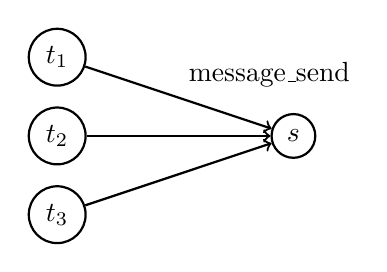
\begin{tikzpicture}
		% formatos
		\tikzstyle{node} = [draw, circle, thick]
		\tikzstyle{arrow} = [->, thick, auto]
		% nodos
		\node [node] (t1)
		{$t_1$};
		\node [node] (t2)	[below of =t1]	{$t_2$};
		\node [node] (t3)	[below of =t2]	{$t_3$};
		\node [node] (s)	[right of =t2, node distance=3cm]
{$s$};
		% relaciones
		\draw [arrow] (t1) to node {message\_send} (s);
		\draw [arrow] (t2) to node {} (s);
		\draw [arrow] (t3) to node {} (s);
	\end{tikzpicture}
	\selectlanguage{spanish}
	\caption{Ejecución de la función $f$ en el servidor}
	\label{fig:mensajes_servicio}
\end{figure}

Se utilizará una función \emph{doReq} que enviará el requerimiento, la
ejecución de la función $f$ al servidor utilizando mensajes, o sea, mediante
\texttt{message\_send}.

\begin{lstlisting}
struct task *server; /* = task_emmit (serverProc); */

/* Mensaje que se pasara al servidor (es el requerimiento) */
typedef struct req
{
  int (*f) (Param *p);
  Param *p;
} Req;

/* Funcion que hace el requerimiento al servidor */
int doReq(int (*f)(Param *p), Param *p)
{
  Req r;
  r.f = f;
  r.p = p;
  return message_send(server, &r);
}

/* Funcion que ejecuta función f de forma secuencial segun se reciben */
int serverProc ()
{
  for(;;) {
    struct task *t;
    Req *pr = (Req *) message_receive (&t, -1);
    int rc = (*pr->f)(pr->p);
    message_reply(t, rc);
  }
}
\end{lstlisting}

\subsection{Implementación de semáforos a partir de mensajes}

\begin{lstlisting}
#define WAIT 1
#define SIGNAL 2

typedef struct
{
  struct task *semTask;
} *Sem;

Sem semMake (int ini) {
  Sem s = (Sem) nMalloc (sizeof(*s));
  s->semTask = task_emmit (semProc, ini);
}

void semWait (Sem s)
{
  int cmd = WAIT;
  message_send(s->semTask, &cmd);
}

void semSignal (Sem s)
{
  int cmd = SIGNAL;
  message_send(s->semTask, &cmd);
}

int semProc (int tickets)
{
  FifoQueue q = MakeFifoQueue();
  for(;;) {
    struct task *t;
    int *pcmd = (int *) message_receive (&t, -1);
    /* Si es un WAIT */
    if(*pcmd==WAIT) {
    	/* Si hay tickets otorgar */
      if(tickets>0) {
        message_reply(t, 0);
        tickets--;
      }
      /* En caso que no hayan tickets encolar */
      else {
        PutObj(q, t);
      }
    }
    /* Si es un SIGNAL */
    else if(*pcmd==SIGNAL) { /* if no es necesario en este caso */
      /* Si la cola esta vacia se aumentan los tickets */
      if(EmptyFifoQueue(q)) {
        tickets++;
      }
      /* Si hay elementos en la cola se despierta */
      else { /* implica tickets = 0 */
        struct task *w = (nTask) GetObj(q);
        message_reply(w, 0);
      }
      message_reply(t,0); /* podria ir antes de verificar la cola */
    }
  }
}
\end{lstlisting}

\section{Monitores de Hoare}

Los \textbf{monitores de
Hoare}\footnote{\url{http://en.wikipedia.org/wiki/Tony_Hoare}} corresponden a
otro tipo de monitores, donde su implementación difiere de la vista
anteriormente. Antes de entrar en su definición y API, una pregunta que aparece
es \textbf{¿por qué se necesitan?}, para responder a esto se verá el caso de la
implementación de semáforos mediante monitores la cual resultará en una
implementación con problemas.

\subsection{Implementación de semáforos a partir de monitores}
\begin{lstlisting}
typedef struct sem
{
  int c;               /* este es el contador para el semaforo */
  struct monitor *m;   /* monitor para controlar el acceso al semaforo */
} *Sem;

Sem semMake (int ini)
{
  Sem s = (Sem) nMalloc (sizeof(*s));
  s->c = ini;
  s->m = monitor_make ();
  return s;
}

void waitSem (Sem s)
{
  monitor_enter (s->m);
  while(s->c==0)
    monitor_wait (s->m);
  s->c--;
  monitor_exit (s->m);
}

void signalSem (Sem s)
{
  monitor_enter (s->m);
  s->c++;
  monitor_notify_all (s->m);
  monitor_exit (s->m);
}
\end{lstlisting}

Pueden existir $n$ hebras que están esperando que otra hebra ejecute un
\texttt{signalSem}, que ejecutará un \texttt{monitor\_notify\_all}. Al ocurrir
esto se despertarán todos las hebras esperando con \texttt{monitor\_wait } y el
primero que lo haga adquirirá el \emph{ticket} que se depositó con
\texttt{signalSem}, mientras que el resto deberá llamar a \texttt{monitor\_wait}
nuevamente. Esto trae dos problemas:

\begin{enumerate}

\item No está garantizado el orden en que se despiertan los procesos al usar
\texttt{monitor\_notify\_all}, por lo cual el semáforo no tendría orden FIFO.

\item Esta implementación es ineficiente debido a los numerosos cambios de
contexto necesarios para que cada uno de los procesos verifique que no hay
\emph{tickets} (a partir del segundo despertado) y se vuelva a dormir.

\end{enumerate}

Los problemas anteriores se evitarían si existiese una forma de despertar solo a
un proceso, y que solo ese proceso tome el \emph{ticket}. Este proceso debiese
ser el primero que se puso en espera con \texttt{monitor\_wait}. Como solución a
esto se debe utilizar \textbf{\texttt{monitor\_notify}} que despertará solo a
una hebra, la primera que se puso a dormir con \texttt{monitor\_wait}.

A pesar de utilizar una cola FIFO en la implementación de \texttt{monitor\_wait}
podría igualmente haber competencia entre procesos, ya que justo cuando se está
despertando a una hebra (y solo a una, por el uso de FIFO) puede existir otra
hebra que está ejecutando justamente un \texttt{monitor\_enter}, en dicho caso
ambas competirían.

Lo interesante es ver si esta solución con \texttt{monitor\_notify} servirá para
todos los casos, veremos a continuación que no sucede así, mediante el ejemplo
del problema del productor consumidor.

\subsection{Problema productor consumidor}

\begin{lstlisting}
void put(Item it)
{
  monitor_enter (ctrl);
  while(c==N)
    monitor_wait (ctrl);
  ...
  monitor_notify_all (ctrl);
  monitor_exit (ctrl);
}
Item get()
{
  monitor_enter (ctrl);
  while(c==0)
    monitor_exit (ctrl);
  ...
  monitor_notify_all (ctrl);
  monitor_exit (ctrl);
}
\end{lstlisting}

Para el ejemplo anterior uno podría, intuitivamente, cambiar los
\texttt{monitor\_notify\_all} por \texttt{monitor\_notify}. Sin embargo, ¿podría
darse la situación en donde hay tanto un productor y un consumidor en un
\texttt{monitor\_wait}? Si un consumidor ejecuta un \texttt{get} y despierta con
\texttt{monitor\_notify} a otra hebra, se esperaría que esa hebra fuese un
productor, pero si hubiera tanto un productor como un consumidor se podría
despertar el consumidor, que al revisar que no hay objetos se dormiría y el
productor, que debiese haber despertado, seguirá durmiendo por que nadie le
avisa que debe producir. ¿Utilizar un monitor para los productores y otro para
los consumidores ayudaría a solucionar el problema recién planteado?, quizás
si, pero en general el trabajo con dos monitores es complicado y propenso a
interbloqueos.

Aquellos problemas donde no sirve simplemente que se despierte al primero que se
fue a dormir, \texttt{monitor\_notify} no será la solución. En muchos casos
\texttt{monitor\_notify\_all} no puede ser eemplazado directamente por un
\texttt{monitor\_notify}. El caso de la implementación de semáforos es uno de
los pocos casos donde funciona, ya que ahí justamente se requiere el orden FIFO
que provee \texttt{monitor\_notify}, despertando al primero que está esperando
por el monitor.

\subsection{Solución de verdad: monitores de Hoare}

Se utilizarán los los tipos de datos \texttt{struct monitor\_condition*}
que básicamente representan una cola de tareas que se administra en orden FIFO.
Estas colas están asociadas al monitor que se está utilizando. En el fondo se
usan los mismos monitores, pero se añade una cola para que esperen los hilos que
se están durmiendo, de esta forma al despertarlos se despierta a las hebras de
una cola específica, no a ``cualquiera'', esto solucionaría el problema del
productor consumidor, donde con \texttt{monitor\_notify} se podía despertar a
cualquiera (productor o consumidor).

¿Se garantiza orden FIFO?, nuevamente no necesariamente, ya que se puede
despertar a un consumidor que estaba durmiendo y justo en ese momento entrar un
nuevo consumidor que ejecuta \texttt{monitor\_enter} y ambos competir por la
propiedad del monitor. Sin embargo los ``wait'' si son en orden FIFO, o sea se
despertará al primero que llamó a \texttt{monitor\_condition\_make}. Es por esta
razón que el \texttt{while} debe seguir estando presente, para seguir evaluando
la condición una vez es despertada la tarea.

\subsubsection{Problema productor consumidor}

Ejemplo del productor consumidor con monitores de Hoare.

\begin{lstlisting}
struct monitor *ctrl;               /* = monitor_make (); */
struct monitor_condition *noempty,  /* = monitor_condition_make (ctrl); */
			*nofull;    /* = monitor_condition_make (ctrl); */
void put(Item it)
{
  monitor_enter (ctrl);
  while(c==N)
    monitor_condition_wait (nofull);
  ...
  monitor_condition_signal (noempty);
  monitor_exit (ctrl);
}
Item get()
{
  monitor_enter (ctrl);
  while(c==0)
    monitor_condition_wait (noempty);
  ...
  monitor_condition_signal (nofull);
  monitor_exit (ctrl);
}
\end{lstlisting}

Existen variantes que pueden implementar
\texttt{monitor\_condition\_signal\_all}, lo cual sería el equivalente a
\texttt{monitor\_notify\_all}.

Este tipo de monitores pueden presentar utilidad en algunos casos, como en este
problema del productor consumidor, sin embargo, en general, se utilizarán los
monitores de Brinch Hansen.

\section{Ejercicios y preguntas}
\begin{enumerate}

\item ¿Por qué utilizar \texttt{while(flag);} como solución en los problemas de
sincronización es incorrecto?. Indique las dos razones.

\item Explique el concepto de espera activa.

\item Explique el concepto de espera pasiva.

\item Considere la solución siguiente para el problema de la cena de
filósofos:

\begin{lstlisting}
void filosofo (int i)
{
  for(;;) {
    comer(i, (i+1)%5);
    pensar();
  }
}
\end{lstlisting}

¿por qué es incorrecta?

\item En el problema de la cena de filósofos, ¿por qué usando semáforos puede
ocurrir interbloqueo? ¿cómo se soluciona con semáforos?.

\item ¿Por qué en el problema de lectores escritores, varios lectores
pueden ejecutarse simultáneamente pero no así los escritores?.

\item Mencione tres características de los semáforos.

\item En semáforos ¿se garantiza el orden en la entrega de los \emph{tickets}?

\item ¿Un monitor puede ser considerado como un semáforo?.

\item ¿Qué operación de monitores hace la diferencia entre un semáforo binario y
un monitor?.

\item Un monitor permite consultar por un invariante sin dejar ``tomado'' el
monitor en caso que este no sea satisfactorio para poder continuar, esto hace
uso de un ciclo \texttt{while}. Este ciclo ¿es espera activa o pasiva?.

\item ¿Para que se utiliza \texttt{monitor\_notify\_all}?.

\item En monitores ¿se garantiza la entrega de la propiedad del monitor?.

\item Indique el patrón de solución de problemas de sincronización usando
monitores.

\item ¿Por qué los monitores pueden producir hambruna?.

\item En mensajes ¿se garantiza el orden en que se procesan los mensajes?.

\item ¿Quién debe responder a un mensaje?.

\end{enumerate}

\section{Referencias}
\begin{itemize}

\item Sistemas Operativos, Segunda Edición, Andrew Tanenbaum, Capítulo 2.2 y
2.3.

\item Sistemas Operativos, Quinta Edición, Abraham Silberschatz y Peter
Baer Galvin, Capítulo 6 y 7.

\item Sistemas Operativos, Segunda Edición, William Stallings, Capítulo 4 y 5.

\end{itemize}
